% !TEX program = lualatex
\documentclass{report}

\usepackage{amsmath}
\usepackage{indentfirst}
\usepackage{graphicx}
\usepackage[margin=2cm]{geometry}
\usepackage{tikz}
\usepackage{hyperref}

\usetikzlibrary{graphs, graphdrawing, matrix, quotes, arrows.meta}
\usegdlibrary{circular}

\renewcommand{\familydefault}{\sfdefault}
\renewcommand{\chaptername}{}
\renewcommand{\labelitemi}{$\bullet$}

\begin{document}
    \tableofcontents
    \chapter{Introduction}
\label{chap:introduction}

    % !TEX program = lualatex
\documentclass{standalone}

% \usepackage{amsmath}
% \usepackage{indentfirst}
\usepackage{graphicx}
% \usepackage[margin=2cm]{geometry}
\usepackage{tikz}
% \usepackage{hyperref}

\usetikzlibrary{graphs, graphdrawing, matrix, quotes, arrows.meta}
\usegdlibrary{circular}

\renewcommand{\familydefault}{\sfdefault}
% \renewcommand{\labelitemi}{$\bullet$}

\begin{document}
\begin{tikzpicture}
    \matrix (m) [matrix of nodes, row sep = 2em, column sep = 2em, nodes = {text depth = 1ex, text height = 2ex, draw, circle, minimum size = 55 pt}]
    {
    ITI & Start Trial & FT & Stimulus & Choice & Reward \\
        &             &    &  Abort   &        &        \\
    };
    \draw [-stealth]
        (m-1-1) edge  ["reset", sloped, font=\small, in=100, out=60, looseness=4] (m-1-1)
        (m-1-1) edge (m-1-2)
        (m-1-2) edge (m-1-3)
        (m-1-3) edge (m-1-4)
        (m-1-4) edge (m-1-5)
        (m-1-5) edge (m-1-6)
        (m-1-6) edge[bend right] (m-1-1)
        (m-1-2) edge["miss", sloped, font=\small] (m-2-4) 
        (m-1-3) edge["miss", sloped, font=\small] (m-2-4) 
        (m-1-4) edge["miss", sloped, font=\small] (m-2-4) 
        (m-1-5) edge["miss", sloped, font=\small] (m-2-4) 
        (m-2-4) edge[bend left] (m-1-1);
\end{tikzpicture}
\end{document}
    \chapter{Bonsai Guidelines}
\label{chap:bonsai}
The implementation of the task described in Chapter \ref{chap:state_machine} was made with the Bonsai visual programming language. The goal of this chapter is to approach some aspects regarding the Bonsai implementation. However, a minimum degree of familiarity with the language will be assumed and the workflow will not be documented node by node.

When the workflow is first opened, the state machine schematized in Figure \ref{fig:state_machine} is easily identifiable. Here are some notes regarding the main workflow:
\begin{itemize}
    \item The states are implemented as SelectMany nodes;
    \item There is an additional SelectMany node that is responsible for outputting data from each trial;
    \item The last nodes of the state machine implementation are what allow the repetition of the workflow and, hence, to start a new trial;
    \item The initialization of variables, distributions and interface with hardware is implemented in GroupWorkflow nodes that aren't part of the state machine.
\end{itemize}

\section{State (SelectMany) Workflow Organization Logic}
\label{sec:state_organization}
It doesn't take much until a Bonsai workflow starts getting complex and, consequently, confusing. In order to improve the readability of the workflow (or at least try), a few guidelines are being followed so that any person that needs to look at the implementation of the task can easily understand it (and/or modify it):
\begin{itemize}
    \item In the main workflow, the inputs and outputs of each SelectMany node (i.e. each state) should be of the type Tuple<Boolean,int>. The idea is that the Boolean gives information regarding the validity of a trial, that is if a True comes out of a state the trial should proceed as planned, otherwise it should abort; and the int indicates the state from where the Tuple came from. Despite not being possible to abort a trial from every state, this guideline is a way to future-proof and standardize data-transfer between states.
    \item Separate independent functionality in a workflow (whether it is the main workflow or one of the SelectMany nodes) should be grouped in GroupWorkflow nodes and displayed in the first line of the workflow.
    \item If some logic is composed of multiple nodes and is used more than once, it should also be grouped in a GroupWorkflow node to avoid repetitions (example: TimestampEvent node).
    \item Since there is a sense of sequentiality of events throughtout the task, different branches of a workflow should be sorted from top to bottom by order of execution when possible.
\end{itemize}

\section{Timestamping Method}
\label{sec:timestamping}
In reaction time experiments, it is of extreme importance to timestamp every event with precision. A reliable way to timestamp each event is by using hardware timestamps (from the Harp Behavior board, to be exact).

Inside the SelectMany nodes where the different states are implemented, it is possible to find a node called TimestampEvent after events that need to be timestamped externally (i.e. non-Harp events). This node consists of a GroupWorkflow which, internally, receives an event from the outside and a hardware timestamp from the Timestamp subject (initialized in the Behavior GroupWorkflow), then ``zips'' both and sends the tuple to the CreateTimestamped node, which converts the tuple into a Bonsai.Harp.Timestamped<T> data type, and finally outputs it to the next node of the workflow. Figure \ref{fig:timestamp_event} shows the inside of the TimestampEvent node.

\begin{figure}[!ht]
    \centering
    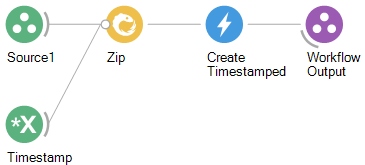
\includegraphics[width=0.3\textwidth]{Figures/timestamp_event.png}
    \caption{TimestampEvent GroupWorkflow ({\color{red} DEPRECATED})}
    \label{fig:timestamp_event}
\end{figure}
    \chapter{Input/Output Files}
\label{chap:io_files}

One of the goals behind this Bonsai workflow is that it is possible to perform similar SLT tasks with small subtleties between them. To achieve this goal, the workflow reads 2 input files ({\color{red} 3 in the future??}) which contain the parameters needed to run the task. The input parameters are divided in 2 ({\color{red} 3 in the future??}) different files: \textit{animal\_settings.json} and \textit{training\_settings.csv} ({\color{red} possible \textit{setup\_settings.json} in the future}). By separating the input parameters in different files, it is possible to define the animal-specific({\color{red}, the setup-specific}) and the task/level-specific parameters independently.

This chapter is dedicated to the description of the file formats as well as of their parameters. In addition to the input files mentioned previously, the format of the output file (which is only one and universal for all tasks ran with this workflow) will also be described here.

\section{Animal-Specific File}
\label{sec:animal_specific}
The animal-specific file is a JSON file which contains information regarding the task that is specific to a certain animal, such as the animal ID number and the session number. Below, it is possible to see an example of this file.
\begin{verbatim}
    {
    "Animal": 1,
    "Box": 2,
    "Session": 53,
    "SessionType": 1,
    "PossibleABLs": [20, 40, 60],
    "CycleILD": 1,
    "Bias": 0.5,
    "FixationBase": 0.01,
    "FixationBaseDelta": 1E-3,
    "FixationBaseTarget": 0.2,
    "FixationExpMean": 0.075,
    "FixationExpMeanDelta": 0.075,
    "FixationExpMeanTarget": 0.075,
    "MinRT": 0.01,
    "RTDelta": 1E-3,
    "RTTarget": 0.15,
    "MaxRT": 10,
    "MaxSamplingTime": [],
    "MinMT": 0.01,
    "MinLNP": 0.01,
    "LNPDelta": 1E-3,
    "LNPTarget": 0.01
}
\end{verbatim}  

The names and order of appearance of the parameters need to be exactly as shown in the example so that Bonsai is correctly able to load the parameters. For the rest of this section, a description of each parameter contained in the animal-specific file will be made.

\subsection*{Animal}
\begin{itemize}
	\item Description: 
	\item Implemented: Yes
\end{itemize}

\subsection*{Box}
\begin{itemize}
	\item Description: 
	\item Implemented: Yes
\end{itemize}

\subsection*{Session}
\begin{itemize}
	\item Description: 
	\item Implemented: Yes
\end{itemize}

\subsection*{SessionType}
\begin{itemize}
	\item Description: 
	\item Implemented: Yes
\end{itemize}

\subsection*{SessionDuration}
\begin{itemize}
	\item Description: The duration of the task ("hh:mm:ss").
	\item Implemented: Yes
\end{itemize}

\subsection*{StartingTrialNumber}
\begin{itemize}
	\item Description: 
	\item Implemented: Yes
\end{itemize}

\subsection*{StartingBlockNumber}
\begin{itemize}
	\item Description: 
	\item Implemented: Yes
\end{itemize}

\subsection*{ABLList}
\begin{itemize}
	\item Description: Possible ABLs to present when DifferentABLs is 1.
	\item Implemented: Yes
\end{itemize}

\subsection*{CycleILD}
\begin{itemize}
	\item Description: Random draw from subcycle only to compute next ILD.
	\item Implemented: Yes
\end{itemize}

\subsection*{Bias}
\begin{itemize}
	\item Description: Left < 0.5, Right > 0.5.
	\item Implemented: No
\end{itemize}

\subsection*{MinFT}
\begin{itemize}
	\item Description: The minimum fixation time (ms).
	\item Implemented: Yes
\end{itemize}

\subsection*{FTDelta}
\begin{itemize}
	\item Description: The increment to make to the constant part of fixation time every non-abort trial (ms).
	\item Implemented: Yes
\end{itemize}

\subsection*{FTTarget}
\begin{itemize}
	\item Description: The target value for the constant part of the fixation time (ms).
	\item Implemented: Yes
\end{itemize}

\subsection*{ExpFTMean}
\begin{itemize}
	\item Description: The mean value of the random part of the fixation time (ms).
	\item Implemented: Yes
\end{itemize}

\subsection*{MinRT}
\begin{itemize}
	\item Description: Minimum amount of time in CNP to wait after the sound presentation starts (s).
	\item Implemented: Yes
\end{itemize}

\subsection*{RTDelta}
\begin{itemize}
	\item Description: The increment to make to RT every non-abort trial (s).
	\item Implemented: Yes
\end{itemize}

\subsection*{RTTarget}
\begin{itemize}
	\item Description: The target value for RT (s).
	\item Implemented: Yes
\end{itemize}

\subsection*{MaxRT}
\begin{itemize}
	\item Description: Maximum amount of time in CNP to wait after the sound presentation starts (s).
	\item Implemented: Yes
\end{itemize}

\subsection*{MaxSamplingTime}
\begin{itemize}
	\item Description: 
	\item Implemented: No
\end{itemize}

\subsection*{MinMT}
\begin{itemize}
	\item Description: Minimum time allowed to move to LNP after leaving CNP (s).
	\item Implemented: Yes
\end{itemize}

\subsection*{MinLNP}
\begin{itemize}
	\item Description: Minimum poke duration in LNP (s).
	\item Implemented: Yes
\end{itemize}

\subsection*{LNPDelta}
\begin{itemize}
	\item Description: The increment to make to LNP time every non-abort trial (s).
	\item Implemented: Yes
\end{itemize}

\subsection*{LNPTarget}
\begin{itemize}
	\item Description: The target for LNP time (s).
	\item Implemented: Yes
\end{itemize}

% \subsection*{PenaltyDurationPress}
% \begin{itemize}
% 	\item Description: Penalty duration upon button press (s).
% 	\item Implemented: No
% \end{itemize}

% \subsection*{PenaltyFlashF}
% \begin{itemize}
% 	\item Description: Penalty flickr frequency (Hz).
% 	\item Implemented: No
% \end{itemize}

% \subsection*{PerformAvg}
% \begin{itemize}
% 	\item Description: Number of trials to average for performance plot.
% 	\item Implemented: No
% \end{itemize}

% \subsection*{FS}
% \begin{itemize}
% 	\item Description: Sampling frequency of IO board.
% 	\item Implemented: No
% \end{itemize}

% \subsection*{FSDiv}
% \begin{itemize}
% 	\item Description: Factor to divide the above to meet performance of code.
% 	\item Implemented: No
% \end{itemize}

% \subsection*{FSSound}
% \begin{itemize}
% 	\item Description: Sampling rate sound card (Hz).
% 	\item Implemented: No
% \end{itemize}

% \subsection*{MinFreq}
% \begin{itemize}
% 	\item Description: Min freq. to band pass (Hz).
% 	\item Implemented: No
% \end{itemize}

% \subsection*{MaxFreq}
% \begin{itemize}
% 	\item Description: Max freq. to band pass (Hz).
% 	\item Implemented: No
% \end{itemize}

% \subsection*{RampTime}
% \begin{itemize}
% 	\item Description: Duration of sound ramp (s).
% 	\item Implemented: No
% \end{itemize}

% \subsection*{SoundDuration}
% \begin{itemize}
% 	\item Description: 
% 	\item Implemented: No
% \end{itemize}

% \subsection*{IBILight}
% \begin{itemize}
% 	\item Description: Lights between blocks or not.
% 	\item Implemented: No
% \end{itemize}

% \subsection*{RightSlope}
% \begin{itemize}
% 	\item Description: 
% 	\item Implemented: No
% \end{itemize}

% \subsection*{RightIntercept}
% \begin{itemize}
% 	\item Description: 
% 	\item Implemented: No
% \end{itemize}

% \subsection*{RCalFactor}
% \begin{itemize}
% 	\item Description: 
% 	\item Implemented: No
% \end{itemize}

% \subsection*{RFVecCal}
% \begin{itemize}
% 	\item Description: 
% 	\item Implemented: No
% \end{itemize}

% \subsection*{LeftSlope}
% \begin{itemize}
% 	\item Description: 
% 	\item Implemented: No
% \end{itemize}

% \subsection*{LeftIntercept}
% \begin{itemize}
% 	\item Description: 
% 	\item Implemented: No
% \end{itemize}

% \subsection*{LCalFactor}
% \begin{itemize}
% 	\item Description: 
% 	\item Implemented: No
% \end{itemize}

% \subsection*{LFVecCal}
% \begin{itemize}
% 	\item Description: 
% 	\item Implemented: No
% \end{itemize}

% \subsection*{RewardOpenL}
% \begin{itemize}
% 	\item Description: The amount of time the left reward port is open (s).
% 	\item Implemented: No
% \end{itemize}

% \subsection*{RewardOpenR}
% \begin{itemize}
% 	\item Description: The amount of time the right reward port is open (s).
% 	\item Implemented: No
% \end{itemize}

% \section{Setup-Specific File}
% \label{sec:setup_specific}

\section{Task/Level-Specific File}
\label{sec:task_specific}
The task/level-specific file is a CSV file which contains the input parameters which are specific to a certain experimental procedure but not dependent on the animal. The choice of using a CSV file to input the task/level-specific parameters is justified by the need to easily define different levels (with different parameter values), since an animal has to be trained to perform a specific task, which is achieved by just adding a new row to the CSV file. The last row of the file is the level in which the animal is considered to be fully trained.

For the rest of this section, a description of each parameter contained in the task/level-specific file will be made for order of appearance. Again, the names and order of appearance of the parameters should be preserved to correctly load the parameters to the workflow.

\subsection*{Level}
\begin{itemize}
	\item Description: 
	\item Implemented: No
\end{itemize}

\subsection*{TrialsPerBlock}
\begin{itemize}
	\item Description: Number of trials of the current block.
	\item Implemented: Yes
\end{itemize}

\subsection*{FixedABL}
\begin{itemize}
	\item Description: ABL value to use when DifferentABLs is 0.
	\item Implemented: Yes
\end{itemize}

\subsection*{DifferentABLs}
\begin{itemize}
	\item Description: Whether to use the ABLs from the ABLList (1) or the FixedABL (0).
	\item Implemented: Yes
\end{itemize}

\subsection*{ABLBlock}
\begin{itemize}
	\item Description: Whether ABLs change only across blocks (1) or not (0).
	\item Implemented: Yes
\end{itemize}

\subsection*{ILDStepSize}
\begin{itemize}
	\item Description: The separation between two consecutive |ILD| values.
	\item Implemented: Yes
\end{itemize}

\subsection*{ILDSteps}
\begin{itemize}
	\item Description: The number of |ILD| values. The final array will contain 2*ILDSteps elements to account for both the positive and the negative ILD values.
	\item Implemented: Yes
\end{itemize}

\subsection*{UseLog}
\begin{itemize}
	\item Description: Whether to use logarithmic steps between consecutive ILD values.
	\item Implemented: Yes
\end{itemize}

\subsection*{LogBase}
\begin{itemize}
	\item Description: The base of the logarithm.
	\item Implemented: Yes
\end{itemize}

\subsection*{IntendedITI}
\begin{itemize}
	\item Description: The intended ITI duration (s).
	\item Implemented: Yes
\end{itemize}

\subsection*{ITIReset}
\begin{itemize}
	\item Description: Whether the ITI partially resets if they try to poke in before it ends.
	\item Implemented: Yes
\end{itemize}

\subsection*{MaxWait}
\begin{itemize}
	\item Description: The maximum allowed time to start the trial (s).
	\item Implemented: Yes
\end{itemize}

\subsection*{UseRT}
\begin{itemize}
	\item Description: Whether the sound stops with the animal leaving the CNP.
	\item Implemented: Yes
\end{itemize}

\subsection*{UseMaxRT}
\begin{itemize}
	\item Description: Whether there is a MaxRT.
	\item Implemented: Yes
\end{itemize}

\subsection*{MaxMT}
\begin{itemize}
	\item Description: The maximum allowed time to move to the LNP (s).
	\item Implemented: Yes
\end{itemize}

\subsection*{AbortPenalty}
\begin{itemize}
	\item Description: The abort penalty time (s).
	\item Implemented: Yes
\end{itemize}

\subsection*{IncorrectPenalty}
\begin{itemize}
	\item Description: The incorrect answer penalty time (s).
	\item Implemented: Yes
\end{itemize}

\subsection*{FixationAbortPenalty}
\begin{itemize}
	\item Description: The fixation abort penalty time (s).
	\item Implemented: Yes
\end{itemize}

\subsection*{UsePerformance}
\begin{itemize}
	\item Description: Whether there is a minimum performance requirement to advance block.
	\item Implemented: Yes
\end{itemize}

\subsection*{CriticalPerformance}
\begin{itemize}
	\item Description: The minimum correct answer ratio required to advance block (if UsePerformance is 1).
	\item Implemented: Yes
\end{itemize}

\subsection*{MaxAborts}
\begin{itemize}
	\item Description: 
	\item Implemented: No
\end{itemize}

\subsection*{RepeatError}
\begin{itemize}
	\item Description: Whether the stimulus is repeated after incorrect responses.
	\item Implemented: Yes
\end{itemize}

\subsection*{RepeatAbort}
\begin{itemize}
	\item Description: Whether the stimulus is repeated after aborts.
	\item Implemented: Yes
\end{itemize}

\subsection*{Speakers}
\begin{itemize}
	\item Description: Whether the animal is using headphones or not (Headphones = 1, Box Speakers = 0).
	\item Implemented: Yes
\end{itemize}

\subsection*{AbortLight}
\begin{itemize}
	\item Description: 
	\item Implemented: No
\end{itemize}

\subsection*{ITILight}
\begin{itemize}
	\item Description: 
	\item Implemented: No
\end{itemize}

\section{Output File}
\label{sec:output_file}
The output file that comes out at the end of a session is also a CSV file. In this case, each row corresponds to a different trial. Since this is the file that contains the data that is going to be analyzed and since some trials may be aborted (and at different stages of the state machine), it may be convenient to understand what certain values for some output parameters mean:
\begin{itemize}
    \item For the output parameters which correspond to a timed event (eg: trial\_duration, ITI\_end, timed\_fix, etc.), if the a trial is aborted before one of those parameters is set, the value written in the output file is 0;
    \item For the response\_poke output parameter, -1 corresponds to the left poke, 1 to the right poke and 0 to an abort.
\end{itemize}

\subsection*{Animal}
\begin{itemize}
	\item Description: 
	\item Implemented: Yes
\end{itemize}

\subsection*{Session}
\begin{itemize}
	\item Description: 
	\item Implemented: Yes
\end{itemize}

\subsection*{SessionType}
\begin{itemize}
	\item Description: 
	\item Implemented: Yes
\end{itemize}

\subsection*{Trial}
\begin{itemize}
	\item Description: 
	\item Implemented: Yes
\end{itemize}

\subsection*{Block}
\begin{itemize}
	\item Description: 
	\item Implemented: Yes
\end{itemize}

\subsection*{TrialsPerBlock}
\begin{itemize}
	\item Description: Number of trials of the current block.
	\item Implemented: Yes
\end{itemize}

\subsection*{TrainingLevel}
\begin{itemize}
	\item Description: 
	\item Implemented: Yes
\end{itemize}

\subsection*{ABL}
\begin{itemize}
	\item Description: 
	\item Implemented: Yes
\end{itemize}

\subsection*{ILD}
\begin{itemize}
	\item Description: 
	\item Implemented: Yes
\end{itemize}

\subsection*{Bias}
\begin{itemize}
	\item Description: Left < 0.5, Right > 0.5.
	\item Implemented: No
\end{itemize}

\subsection*{LeftAmp}
\begin{itemize}
	\item Description: 
	\item Implemented: No
\end{itemize}

\subsection*{RightAmp}
\begin{itemize}
	\item Description: 
	\item Implemented: No
\end{itemize}

\subsection*{WaveformL}
\begin{itemize}
	\item Description: The index of the sound played in the left speaker during the current trial.
	\item Implemented: No
\end{itemize}

\subsection*{WaveformR}
\begin{itemize}
	\item Description: The index of the sound played in the left speaker during the current trial.
	\item Implemented: No
\end{itemize}

\subsection*{TrialStart}
\begin{itemize}
	\item Description: Trial start timestamp (s).
	\item Implemented: Yes
\end{itemize}

\subsection*{TrialEnd}
\begin{itemize}
	\item Description: Trial end timestamp (s).
	\item Implemented: Yes
\end{itemize}

\subsection*{TrialDuration}
\begin{itemize}
	\item Description: Duration of the trial (s).
	\item Implemented: Yes
\end{itemize}

\subsection*{IntendedITI}
\begin{itemize}
	\item Description: The intended ITI duration (s).
	\item Implemented: Yes
\end{itemize}

\subsection*{ITIStart}
\begin{itemize}
	\item Description: ITI start timestamp (s).
	\item Implemented: Yes
\end{itemize}

\subsection*{ITIEnd}
\begin{itemize}
	\item Description: ITI end timestamp (s).
	\item Implemented: Yes
\end{itemize}

\subsection*{TimedITI}
\begin{itemize}
	\item Description: Duration of the ITI (s).
	\item Implemented: Yes
\end{itemize}

\subsection*{MaxWait}
\begin{itemize}
	\item Description: The maximum allowed time to start the trial (s).
	\item Implemented: Yes
\end{itemize}

\subsection*{TimeToCNP}
\begin{itemize}
	\item Description: The amount of time it took for the animal to poke in the CNP (s).
	\item Implemented: Yes
\end{itemize}

\subsection*{BaseFT}
\begin{itemize}
	\item Description: The constant part of the fixation time (ms).
	\item Implemented: Yes
\end{itemize}

\subsection*{ExpFTMean}
\begin{itemize}
	\item Description: The mean value of the random part of the fixation time (ms).
	\item Implemented: Yes
\end{itemize}

\subsection*{IntendedFT}
\begin{itemize}
	\item Description: The intended FT duration for the trial (ms).
	\item Implemented: Yes
\end{itemize}

\subsection*{TimedFT}
\begin{itemize}
	\item Description: The actual FT duration (s).
	\item Implemented: Yes
\end{itemize}

\subsection*{BaseRT}
\begin{itemize}
	\item Description: Minimum amount of time in CNP to wait after the sound presentation starts (s).
	\item Implemented: Yes
\end{itemize}

\subsection*{MaxRT}
\begin{itemize}
	\item Description: Maximum amount of time in CNP to wait after the sound presentation starts (s).
	\item Implemented: Yes
\end{itemize}

\subsection*{TimedRT}
\begin{itemize}
	\item Description: The amount of time the animal waited in the CNP after the sound presentation started (s).
	\item Implemented: Yes
\end{itemize}

\subsection*{MaxMT}
\begin{itemize}
	\item Description: The maximum allowed time to move to the LNP (s).
	\item Implemented: Yes
\end{itemize}

\subsection*{TimedMT}
\begin{itemize}
	\item Description: The amount of time it took for the animal to poke in a LNP (s).
	\item Implemented: Yes
\end{itemize}

\subsection*{IntendedLNP}
\begin{itemize}
	\item Description: Minimum poke duration in LNP (s).
	\item Implemented: Yes
\end{itemize}

\subsection*{TimedLNP}
\begin{itemize}
	\item Description: The amount of time the animal kept poking the LNP (s).
	\item Implemented: Yes
\end{itemize}

\subsection*{ResponsePoke}
\begin{itemize}
	\item Description: The side (Left = -1, Right = 1, Abort = 0) that the animal considered the sound was played the loudest.
	\item Implemented: Yes
\end{itemize}

\subsection*{Success}
\begin{itemize}
	\item Description: Whether the animal got the answered correctly (1) or not (0).
	\item Implemented: Yes
\end{itemize}

\subsection*{AbortEvent}
\begin{itemize}
	\item Description: Whether the trial aborted (1) or not (0).
	\item Implemented: Yes
\end{itemize}

\subsection*{RepeatTrial}
\begin{itemize}
	\item Description: Whether this trial should be repeated (1) or not (0).
	\item Implemented: Yes
\end{itemize}

\subsection*{BlockPerformance}
\begin{itemize}
	\item Description: The ratio of right answers to non-abort trials.
	\item Implemented: Yes
\end{itemize}

\subsection*{BlockAbort}
\begin{itemize}
	\item Description: The ratio of abort trials to the total number of trials.
	\item Implemented: Yes
\end{itemize}

\subsection*{LEDTrial}
\begin{itemize}
	\item Description: 
	\item Implemented: No
\end{itemize}

\subsection*{TimedLED}
\begin{itemize}
	\item Description: 
	\item Implemented: No
\end{itemize}

\subsection*{LEDPowerL}
\begin{itemize}
	\item Description: 
	\item Implemented: No
\end{itemize}

\subsection*{LEDPowerR}
\begin{itemize}
	\item Description: 
	\item Implemented: No
\end{itemize}

\subsection*{Box}
\begin{itemize}
	\item Description: The number of the box where the task was conducted.
	\item Implemented: Yes
\end{itemize}


    % \input{Chapters/iti.tex}
    % \input{Chapters/start_trial.tex}
    % \input{Chapters/fixation_time.tex}
    % \input{Chapters/stimulus.tex}
    % \input{Chapters/choice.tex}
    % \input{Chapters/reward.tex}
    % \input{Chapters/abort.tex}
    % \input{Chapters/io_files.tex}
\end{document}